\input{chapter-header.tex}
% ===========================================================================
\part{State of the Art}
% ===========================================================================

%Software inevitable changes and we need to provide with the tools and methodologies that support such changes~\cite{Nier08b}. However, production-ready applications are not usually change-aware. These applications should be either engineered from scratch with change in mind, or a lot of reengineering effort should be invested in them to support change. Making deep modifications to a language runtime can be a cumbersome task.

% ===========================================================================
%\newpage
% ===========================================================================

\chapter{Application Runtime Manipulation}
\chaplabel{state_modifying}
\minitoc

Generating an application runtime requires the basic ability to manipulate such runtime \eg create and modify classes and methods; instantiate objects; begin and stop threads in it. This chapter explores the state of the art on application runtime manipulation. We identify three main concerns that arise when we attempt to modify an application runtime~(Section \ref{sec:bootstrapping_problems}): how easily a change can be applied to a language runtime, how coupled are the application runtime and \VM concerns, and what is the existing tool support to modify such application runtime.

Based on those concerns, we defined a criterion to evaluate existing application runtime manipulation solutions~(Section \ref{sec:runtime_modification_criteria}). We also classified the different techniques for application runtime manipulation in three main categories:

\begin{description}

\item[Reflection models.] The literature presents several language runtime manipulation solutions based on metaprogramming and \emph{reflection}~(Section \ref{sec:related_work_changing}). These metaprogramming models allow either the modification of the language interpreter semantics or the scoping of modifications with one main objective: performing such modifications safely \ie without breaking the application runtime they are running on.

\item[Metacircular runtimes.] Metacircular runtimes aim at easing the modification of a runtime by means of simplifying the language-\VM relation for development~(Section \ref{sec:metacircular_runtimes}). This simplification comes usually by expressing a \VM in the same language it interprets at the end. Metacircular runtimes mostly focus on the simplification of complexity in \VM technology and not on the manipulation of the language runtime elements.

\item[Virtualization techniques.] Virtualization techniques applied to application runtimes are used for application control and manipulation~(Section \ref{sec:background_virtualization_techniques}). Application co-existence allows the modification of an application without affecting others. Application manipulation provides control on an application's life cycle and its internal representation.

\end{description}

\section{Concerns of Application Runtime Manipulation} \label{sec:bootstrapping_problems}

We identify three main concerns when we aim at changing or replacing an application and language runtime. First, how flexible its language runtime is to be changed and adapted without running into inconsistent states. Second, how clear is the separation between the \VM and language concerns to extract the language concerns. Finally, what are the abstraction level and the tool support needed to manipulate an application runtime.


\subsection*{Flexibility to Safely Change a Language Runtime}

The \VM is often the component in charge of initializing the application runtime and particularly the language runtime. This decision is indeed practical as the \VM can safely initialize the language structures, solve the language bootstrapping issues avoiding recursions~\cite{Kicz91a}~(\eg create the first class or the first string without a class) and ensure the created language runtime complies to its execution model. This coupling is indeed necessary to run a program but does often remain hidden in hardcoded assumptions. A consequence of this is that the \VM fixes the initial structures of the language runtime. Figure \ref{code:ruby_hierarchy} illustrates this problem: Ruby's initial class hierarchy is imprinted inside the \VM code, fixing \ct{BasicObject} as the top superclass and followed by \ct{Object}, \ct{Module} and \ct{Class} respectively\footnote{Taken from the version 2.1 of the Ruby VM in \url{http://svn.ruby-lang.org/repos/ruby}}.

\begin{figure}[ht!]
\begin{code}
void Init_class_hierarchy(void) {
    rb_cBasicObject = boot_defclass("BasicObject", 0);
    rb_cObject = boot_defclass("Object", rb_cBasicObject);
    rb_cModule = boot_defclass("Module", rb_cObject);
    rb_cClass =  boot_defclass("Class",  rb_cModule);

    rb_const_set(rb_cObject, rb_intern("BasicObject"),rb_cBasicObject);
    RBASIC_SET_CLASS(rb_cClass, rb_cClass);
    RBASIC_SET_CLASS(rb_cModule, rb_cClass);
    RBASIC_SET_CLASS(rb_cObject, rb_cClass);
    RBASIC_SET_CLASS(rb_cBasicObject, rb_cClass);
}
\end{code}
\caption{\textbf{Code of the Ruby VM that initializes the class hierarchy (excerpt).} The VM code fixes the language class hierarchy.\label{code:ruby_hierarchy}}
\end{figure}

A second problem arises as the \VM includes code to manipulate objects that belong to the application runtime, introducing a duplication between the \VM code and the language code. 
To illustrate this second problem, let us consider the code to the left of Figure~\ref{code:logic_dup} that creates a \ct{Dictionary} object~(a hash map object) in Smalltalk. If our language runtime is defined by a \ct{Dictionary} object keeping \eg a map of global objects, we must execute that code to create the corresponding instance during the language initialization. However, since the language runtime and the \VM are in the middle of their initialization, the \VM cannot execute this code as it is, and thus it cannot enforce its own invariants. Production \VMs will provide an alternative low-level representation of the same code respecting the same invariants, exemplified at the right of the same figure. This introduces a redundancy: the \VM and the language have different code to honor the same invariants.

\begin{figure}[ht]
\begin{subfigure}{.5\linewidth}
\begin{code}
Dictionary class>>new: n
    ^ self new initialize: n

Dictionary>>initialize: n
    "Initialize array to an array size of n"
    array := Array new: n.
    tally := 0
\end{code}
\end{subfigure}
\begin{subfigure}{.5\linewidth}
\begin{code}
void* createDictionaryWithSize(int n){
    void* dictionary, internalArray;
    dictionary = instantiate("Dictionary");
    internalArray := instantiate("Array", n);
    setInstanceVariable(dictionary, 1, internalArray);
    setInstanceVariableInt(dictionary, 2, 0);
    return dictionary;
}
\end{code}
\end{subfigure}
\caption{\textbf{Code to create a \ct{Dictionary} object.} To the left, the code is written in Smalltalk and used by the application runtime. To the right, a C function duplicates this behavior at the \VM level.\label{code:logic_dup}}
\end{figure}


%This execution model is often less restrictive than the object models of the language's that run on top of them. For example, the Smalltalk and Ruby \VMs require for each object in the system to have a class, and each class a superclass, but there is no need for metaclasses.

Once the application runtime is initialized, reflective languages~\cite{Smit84a,Deme95a} such as LISP or Smalltalk provide means to modify themselves at runtime. These languages are based on a reflective architecture presenting the notion of causal connection~\cite{Maes87a}: a link between a programming element and its representation that keeps both in synchronization. However, as these languages contain meta-circular definitions in their kernel~\cite{Chib96a}, this can result in a metastability problem \ie a change in the language runtime may introduce a meta-call recursion and make the system unusable~\cite{Kicz91a}.% In this context, Reflectivity~\cite{Denk08b} is a framework that scopes reflection to avoid meta-call recursions.  Reflectivity succeeds to control behavioural reflection by accounting the level of \emph{metaness} of the execution in a program and executing reflective operations when it is in the correct meta-level. The main limitation of Reflectivity is that it does not allow structural reflective changes in the language runtime.

Finally, snapshot-based languages offer different means to evolve a language runtime. Instead of being reinitialized each time we need it, the state of the whole graph of objects that denotes the running program can be suspended and saved as a snapshot in a file. Later on, the program in this snapshot can be restarted from the point it was suspended. As a consequence of this persistency property, some snapshot-based languages such as Squeak~\cite{Inga97a} or Pharo~\cite{Blac09a} do not have the infrastructure to be reinitialized from scratch. Indeed, their current deliverable snapshots are the result of a chain of side effects (updates and migrations) applied to the original Smalltalk-80 snapshot. Thus, even if we can change the application runtime during execution, they cannot ensure a reproducible initial state for their users.

\subsection*{Separation of \VM and Language Concerns}

The unclear interface between the language and the \VM makes it difficult to recognize whether a piece of code in the \VM belongs to a \VM concern or a language one. This causes undesirable temporal couplings between these two elements and prevents us from extracting and replacing the application runtime by another one.
To illustrate this problem, Figure \ref{code:jikes_vm_initialization} shows an excerpt of the JikesRVM\footnote{Taken from the version 3.1.3 of the JikesRVM in \url{http://sourceforge.net/projects/jikesrvm}}~\cite{Alpe00a}. In this example, the memory manager is initialized in the middle of the initial class loading phase. These memory manager calls are indeed needed to avoid the collection of objects during the initialization. However, it is necessary to call it after some specific classes are initialized and not before.

\begin{figure}[ht]
\begin{code}
private static void finishBooting() {
    ...
    MemoryManager.postBoot(); //Memory management
    ...
    runClassInitializer("java.lang.Runtime");
    runClassInitializer("java.lang.System");
    runClassInitializer("sun.misc.Unsafe");
    ...
    MemoryManager.fullyBootedVM(); //Memory management
    ...
    runClassInitializer("java.util.logging.Level");
    runClassInitializer("gnu.java.nio.charset.EncodingHelper");
}
\end{code}
\caption{\textbf{Code of the JikesRVM that loads and initializes the initial classes of the runtime (excerpt).} The code performing the initial class loading is mixed with the code that initializes the memory manager of the \VM.\label{code:jikes_vm_initialization}}
\end{figure}

Snapshot-based languages, on the other hand, show that language initialization and \VM initialization can be orthogonal. Indeed, languages such as Pharo, LISP or the V8 flavor of Javascript can restart their system from a snapshot. The \VM loads atomically the snapshot and binds it to the current executing \VM. Loading a snapshot clarifies the \VM startup steps as it replaces the runtime initialization phase. Moreover, as long as the snapshot satisfies the \VM execution model, it can run any language model, as it is the case of Pharo and Newspeak that run on the same \VM.

%Other snapshot-based languages such as GNU-Smalltalk or the V8 flavor of Javascript possess both mechanisms: they recreate the language runtime from scratch, and can also restart from a snapshot. In the case of V8, the snapshot was chosen with performance in mind, to avoid parsing and recreation on client-side machines.

%\item[The \VM-Language interface is unclear.]
%For example, the \VM assumes how objects are structured in the runtime to manipulate them: the amount and size of their instance variables, object headers, special kind of object references~(\eg weak references). The \VM also needs access to some well-known objects to run code: this is the case for example of \ct{nil}, \ct{true} and \ct{false} objects. Another example of a tight coupling are the callbacks \VM-language, where the \VM can trigger some specific code on the language to notify it from some event.

\subsection*{Abstraction Level and Tool Support}

When defining the language runtime at the \VM level, we rely on the tools and abstractions available to develop the \VM to change the language. That means that the language developer uses often low-level abstractions to express higher-level concerns. This \emph{mismatch} impacts on the \VM/language developer efficiency, as the tools are not adequate for the task to accomplish. This problem is indeed aggravated with the complexity of such pieces of software, including elements such as the \GC or the JIT that cross-cut every \VM concern.

Indeed the developer would benefit from the productivity that a high-level language brings. In this sense, reflective languages support naturally the usage of the language abstractions and tools to modify the language runtime. Reflective languages benefit from the reification of the language concepts to be able to change them from the language itself. Languages such as Smalltalk show how debuggers and code browsers can be built using such features\gp{cite}.

%To attack these problems, many programming systems have found desirable to follow the principles of \emph{high-level low-level programming} \ie expressing low-level concerns using high-level languages~\cite{Fram09a}. High-level low-level programming pursues the objective of simplifying the complexity of programming systems. By using a high-level language to describe the low-level world the developer benefits from their abstraction power and tooling of the first one. A clear example of this fact is the metacircular \VM field, where many projects whose goal is to write \VMs in a high-level language have blossomed in the last years~\cite{Wimm13a,Alpe00a,Verw11a,Inga97a,Unga05a,Rigo06a}. These projects are biased to \VM building techniques and not to the initialization of the languages that run on top of them.

\section{Evaluation Criteria}\label{sec:runtime_modification_criteria}

This section presents the features we consider relevant to include in a runtime manipulation solution. These features serve as criteria to compare the state of the art we selected in the following sections.

\begin{description}

\item[Manipulate Objects.] An ideal application runtime manipulation must provide access to objects. It should support class instantiation, and the manipulation of such objects, including access to their fields.
\item[Manipulate Language Elements.] An application runtime manipulation solution must support the creation and modification of elements that are part the language runtime \eg create and modify of classes and methods.
\item[Manipulate Execution Elements.] An application runtime manipulation solution must provide support to manipulate elements related to a program's execution \eg the creation, pausing and resumption of threads; the introspection of such threads to understand a program's execution.

\item[Safety.] An ideal application runtime manipulation solution must guarantee that both incorrect modifications cannot be applied, and that correct modifications can be safely applied without leaving the system in an inconsistent state.

\item[User abstraction level.] An ideal application runtime manipulation solution must provide its user with the possibility to express its manipulations in a high-level language. In such a way, users can benefit from the abstractions and expressiveness of such a language.

\item[API abstraction level.] The API of an ideal application runtime manipulation solution must provide the abstractions to manipulate the application runtime in terms of the runtime's constructions.

\item[Separation of concerns.] The solution should clearly separate \VM and language concerns to avoid transmitting to the language developer the complexities of \VM technology such as the \GC or the JIT compiler.

\end{description}

In the following sections we explore and compare three different categories of solutions that pursue different kind of application runtime manipulation. This comparison is based on the criteria defined in this section.

\section{Reflection and Metaprogramming Models}\label{sec:related_work_changing}

Reflection is the capability of a program to reason about and act upon itself~\cite{Maes87a}.
Typically we distinguish two forms of reflective access: structural and behavioral~\cite{Male96b}.
Structural reflection is concerned with the static structure of a program, while behavioral reflection focuses on the dynamic part of a running program.
Orthogonally to the previous categorization we distinguish between introspection and intercession.
Introspection refers to the access to a particular reified representation of a program's element, whereas for intercession we mean to alter the reified representation.

\begin{description}
\item[Structural Reflection.] Structural reflection refers to the access to the static structure of a program.
A typical example\footnote{Throughout this dissertation we use \PH code examples. The syntax and the basic semantics are explained in Appendix \ref{appendixa}} is to access the class of an object at runtime.

\begin{code}
'a string' class.
\end{code}

An example of structural intercession is to reflectively modify an instance variable of an object.

\begin{code}
aCar instVarNamed: #driver put: Person new.
\end{code}

\item[Behavioral Reflection.] Behavioral Reflection means to directly interact with the running program.
For instance this includes reflectively activating a method.

\begin{code}
#Dictionary asClass perform: #new
\end{code}

Another more complex example to dynamically switch the execution context and resend the current method with another receiver.

\begin{code}
thisContext restartWithNewReceiver: Object new 
\end{code}

Accessing the receiver of the current method through the execution context is an example of behavioral introspection.

\begin{code}
thisContext receiver. 
\end{code}
\end{description}

There is not always a clear separation between the two types of reflection.
For instance adding new methods requires structural reflection.
At the same time, adding a new method alters the future program execution, implying that it is also behavioral reflection.
Typically we see that behavioral reflection stops at the granularity of a method.
For instance in \PH by default it is not possible to directly alter the execution on a sub-method level~\cite{Denk06a}.

Reflection provides by default most of the characteristics that we need for runtime manipulation, such as the ability to manipulate the execution of a program or the objects themselves.
In the following sections we present several existing models implementing reflective behavior, and for each of them we put emphasis on their weaknesses and strengths.

\subsection*{\textsc{Tower of Interpreters Model}}

The original model of reflection as defined by Smith~\cite{Smit82c} is based on meta-level interpretation. A program is interpreted by an interpreter, which is interpreted by a meta-interpreter and so on, possibly \emph{ad infinitum}. This leads to a tower of interpreters, where each level defines the semantics of the program~(interpreter of application) it interprets~(Figure \ref{fig:tower_of_interpreters}).

\begin{figure}[ht]
\begin{center}
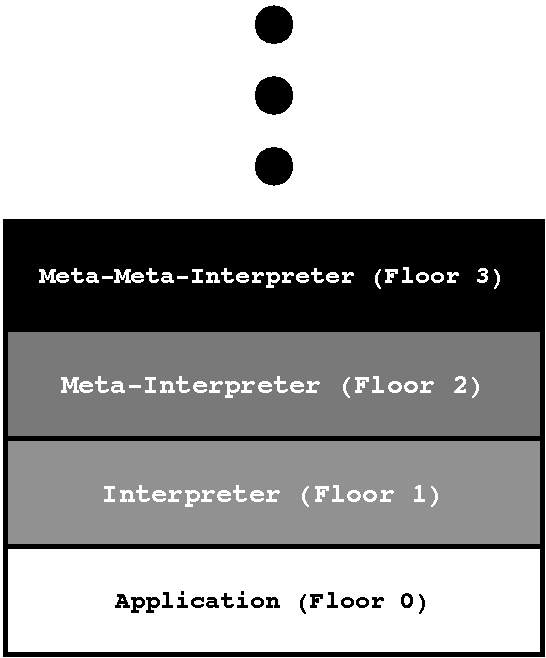
\includegraphics[width=.5\linewidth]{tower_of_interpreters}
\caption{\textbf{The theoretical tower of interpreters model.} Each floor interprets the floor below itself.\label{fig:tower_of_interpreters}
% (a)The host language and (b)the guest language contain each one their own classes and objects. The guest language resides inside the host language during the bootstrap; (c)the builder, a program written in the host language, reifies the bootstrap process itself and bootstraps the guest language given a (d)source code specification.
 }
\end{center}
\end{figure}

The tower of interpreters presents a model where one can define and redefine the semantics of the program it is executing. We can modify the behavior of our program~(in the floor zero) by jumping one level above it in the tower and modifying the interpreter running in that floor. In the same sense, we can jump one level above this interpreter to change also its behavior and so on. This allows the \emph{indirect modification} of a program's behavior \ie a change in an interpreter in a level \emph{n} changes the behavior of the interpreter in the level \emph{n - 1}, which impacts on the interpreter below it and so on, up to the base level.

Smith's tower of interpreters model is flexible and coherent regarding the manipulation of the reflective behavior of a program. The tower does not present a limit on the amount of interpreters we can stack, presenting a problematic infinite potential. This idea collides with the non-infinite resources in current hardware. On one hand, limited memory prevents us to have a tower of infinite interpreters running at the same time. On the other hand, above certain limit of interpreters, this approach becomes too slow and impractical, as discussed in \cite{Male96b,Male96c,Male96d}. We will show in the following subsections other reflective models that try to overcome these deficiencies while trying to keep some of the good properties of this model.

\subsection*{\textsc{Black}}

Black is a reflective language based on Scheme that mimics the infinite tower of interpreters with the goal to make it practical. Its model is based on the same idea as the reflective tower: the base level is interpreted by an interpreter, which is interpreted by a meta-interpreter and so on. The main difference between the original tower of interpreters and the model presented by Black is that the latter avoids the infinite regression, making the model practical in finite resource machines.

Black avoids the infinite regression by limiting the real levels of interpretation: there is only one level of interpretation. For the rest of the levels, Black  introduces a difference between directly-executed code in contrast with interpreted code. Directly-executed code is code that is executed by the machine, where no interpretation steps are involved. Then, the base-level application is the only interpreted code in the application. The rest of the tower, including the first interpreter, is implemented and executed directly in machine code~(Figure \ref{fig:black_tower}).

\begin{figure}[ht]
\begin{center}
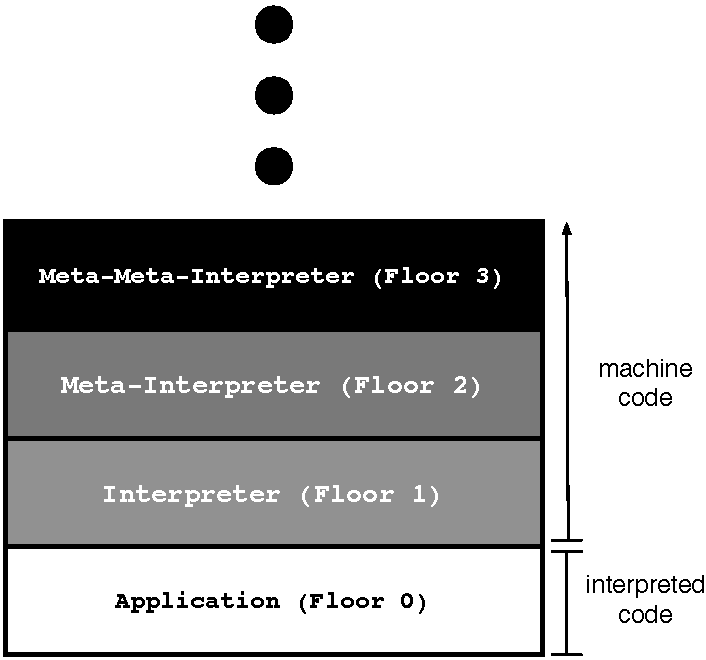
\includegraphics[width=.6\linewidth]{black_tower}
\caption{\textbf{Black model of interpreters.} Only the application level is interpreted. The levels above are directly executed on the machine.\label{fig:black_tower}
% (a)The host language and (b)the guest language contain each one their own classes and objects. The guest language resides inside the host language during the bootstrap; (c)the builder, a program written in the host language, reifies the bootstrap process itself and bootstraps the guest language given a (d)source code specification.
 }
\end{center}
\end{figure}

By limiting the levels of interpretation, the model presented by Black forbids \emph{indirect modification}. Changing the interpreter in a level \emph{n} above the first level does not impact any more the interpreters below it, as they are directly-executed in the machine and not by the modified interpreter. Black supports, however, the modification of the first level of interpretation with the introduction of hooks inside the machine code. A hook detects whether a function in the interpreter~(written in directly-executed code) is changed, and interprets it by a meta-level interpreter written also in directly executed code. Hooks degrade the performance in comparison with a non-hooked interpreter, but it enables to change and specialize the behavior of the directly-executed code.

\subsection*{\textsc{Reflectivity: scoping reflection in Reflective Architectures}}

To enable reflection in mainstream languages such as Java, Ruby or JavaScript, the tower of interpreters is replaced by a reflective architecture~\cite{Maes87a}. Instead of relying on a stack of interpreters interpreting each the level below it, a reflective architecture relies on the idea of \emph{causal connection} \ie the programming language incorporates structures that represents aspects of itself~(\eg classes, objects), in such a way that if one structure changes the aspect it represents is updated accordingly, and vice-versa.


In languages presenting reflective architectures, reflection is controlled by meta-objects that share a same environment with the objects they reflect upon.
One problematic corollary of this is that meta-objects rely on the same code and infrastructure as the objects they reflect upon \eg if a class stores its subclasses in a \ct{Set}, changing the  implementation of \ct{Set} impacts the reflective behavior in addition of the base-application behavior.
Therefore there is a risk of infinite meta-recursion when the meta-level instruments code that it relies upon~(Figure \ref{fig:reflectivity_meta_recursion}).

\begin{figure}[ht]
\begin{center}
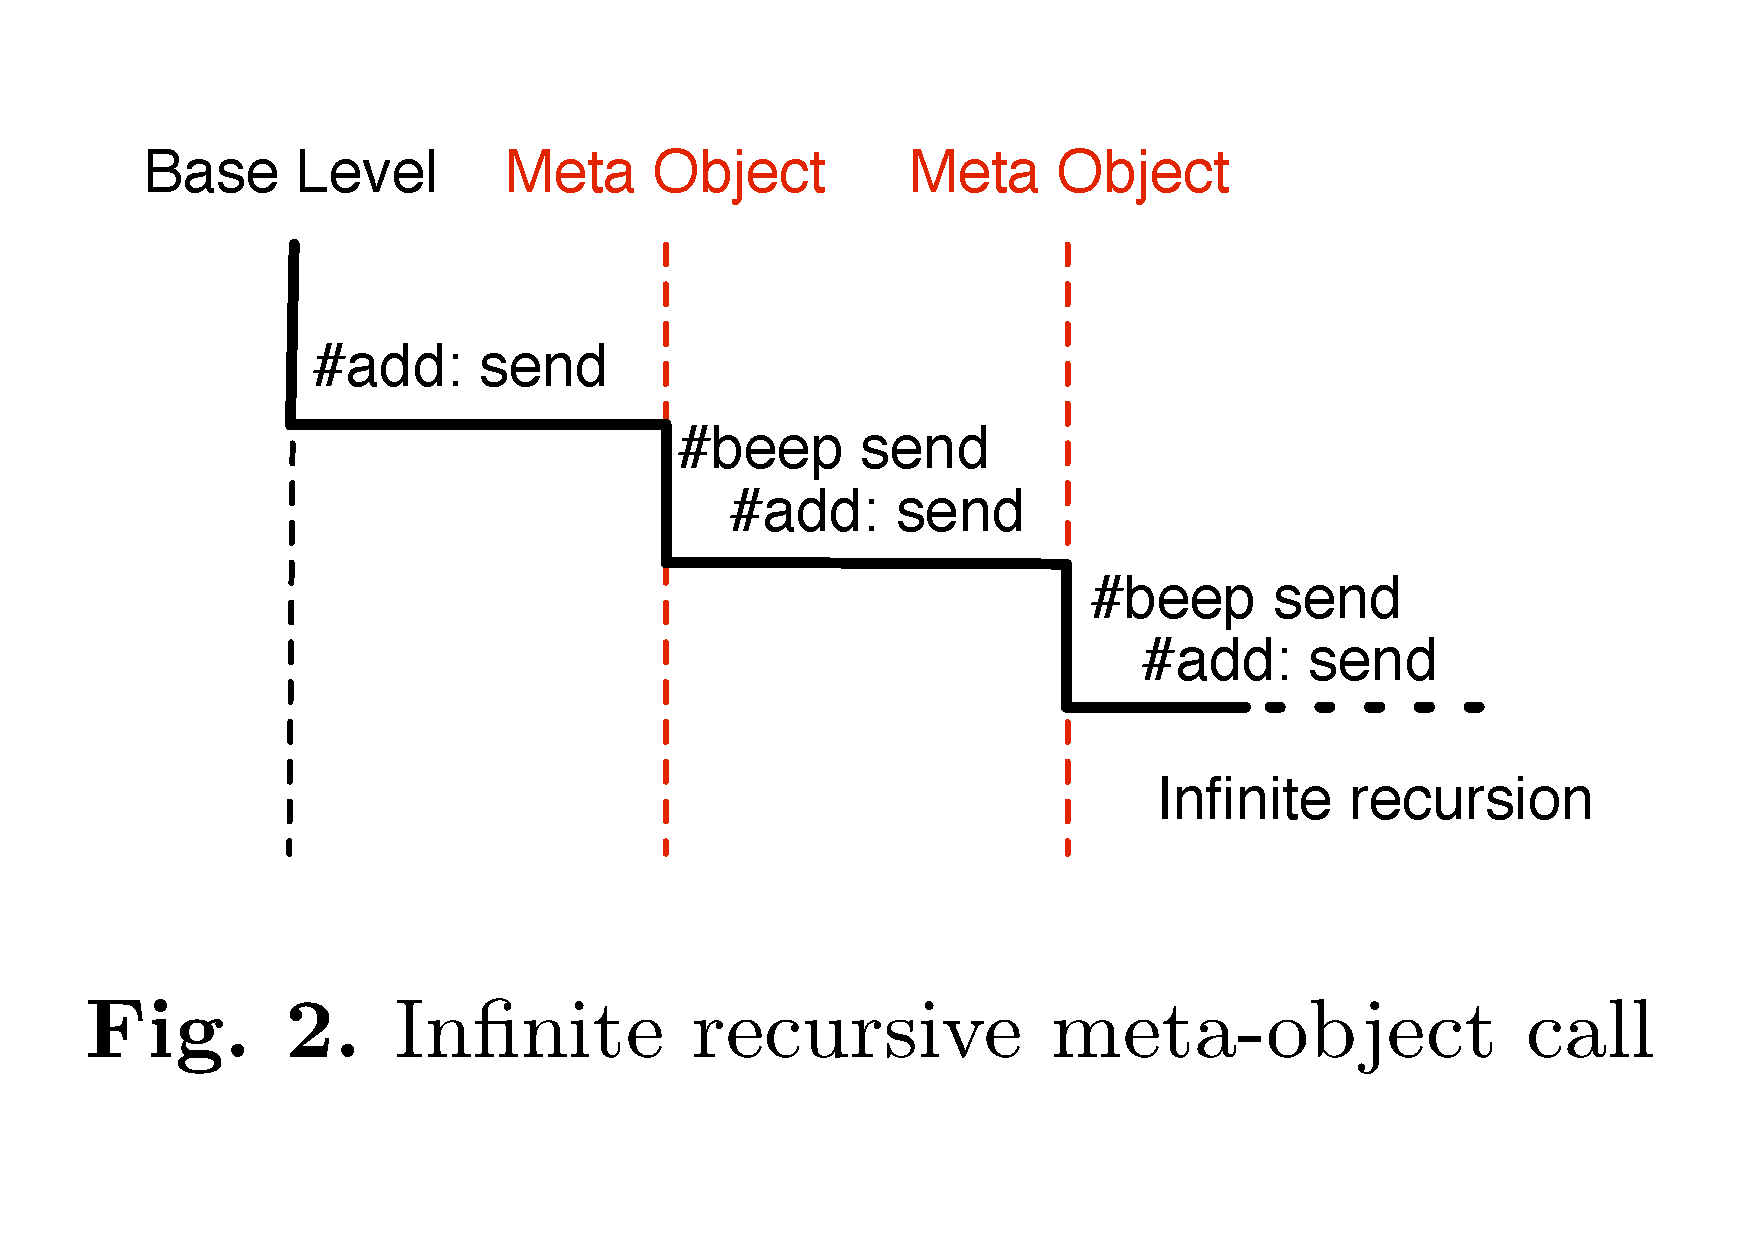
\includegraphics[width=.6\linewidth]{reflectivity_meta_recursion}
\caption{\textbf{Meta level recursion in reflective architectures.}\label{fig:reflectivity_meta_recursion}
% (a)The host language and (b)the guest language contain each one their own classes and objects. The guest language resides inside the host language during the bootstrap; (c)the builder, a program written in the host language, reifies the bootstrap process itself and bootstraps the guest language given a (d)source code specification.
 }
\end{center}
\end{figure}

Denker et al. partially solve this problem in Reflectivity~\cite{Denk08b}. Reflectivity is a reflective framework that avoids meta-recursions by tracking the degree of metaness of the execution context. In each reflective call, the \ct{MetaContext} object is activated and it accounts for the meta-level jump. Likewise, when the reflective call returns, the \ct{MetaContext} is deactivated. Using the accounted meta-level jumps of the \ct{MetaContext}, meta-objects do only reflect on objects of a lower metaness~(and not greater or equal metaness). Thus, it simulates the semantics of an infinite tower of distinct interpreters while there is only one of them that scopes the meta-operations using the accounted meta-level~(Figure \ref{fig:reflectivity_avoid_meta_recursion}).

\begin{figure}[ht]
\begin{center}
\begin{subfigure}{.45\textwidth}
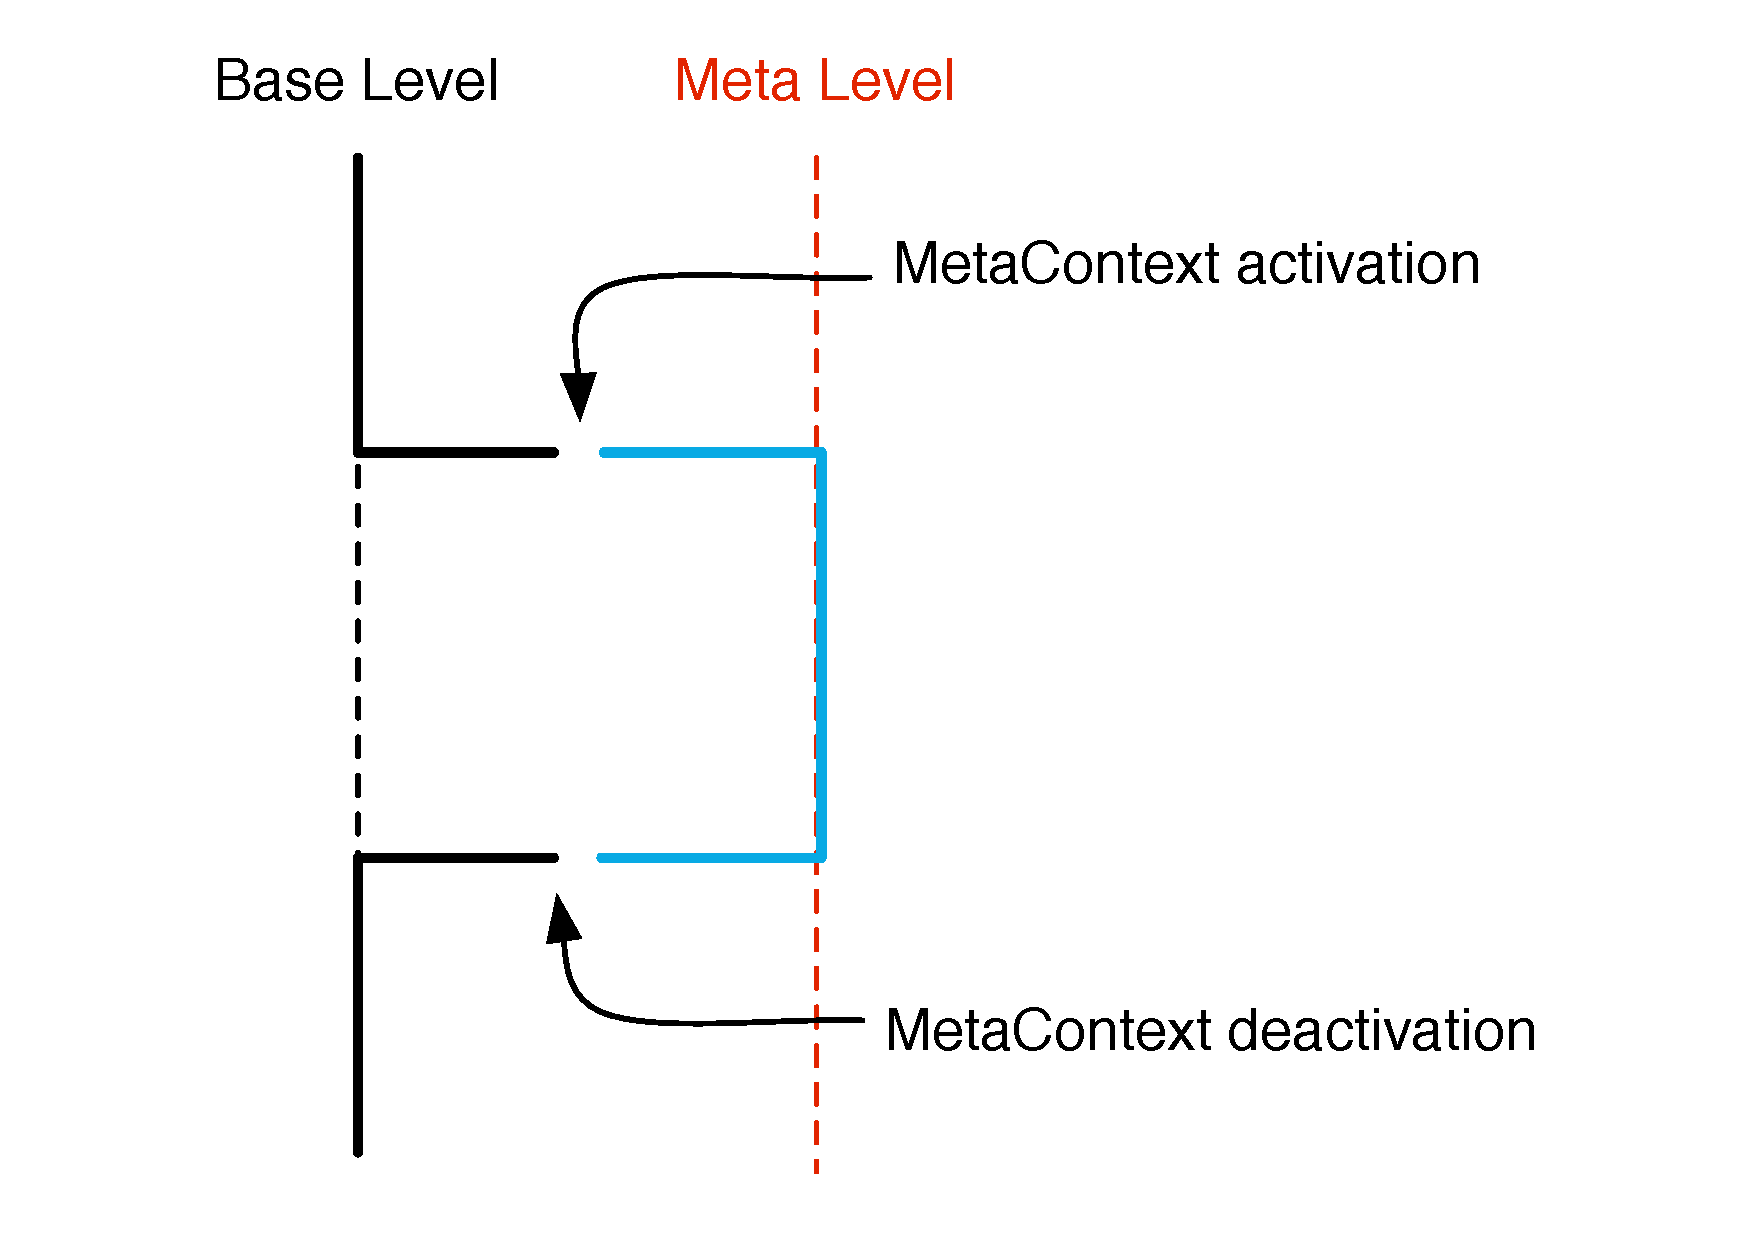
\includegraphics[width=1\linewidth]{reflectivity_metaness_accounting}
\end{subfigure}
\begin{subfigure}{.45\textwidth}
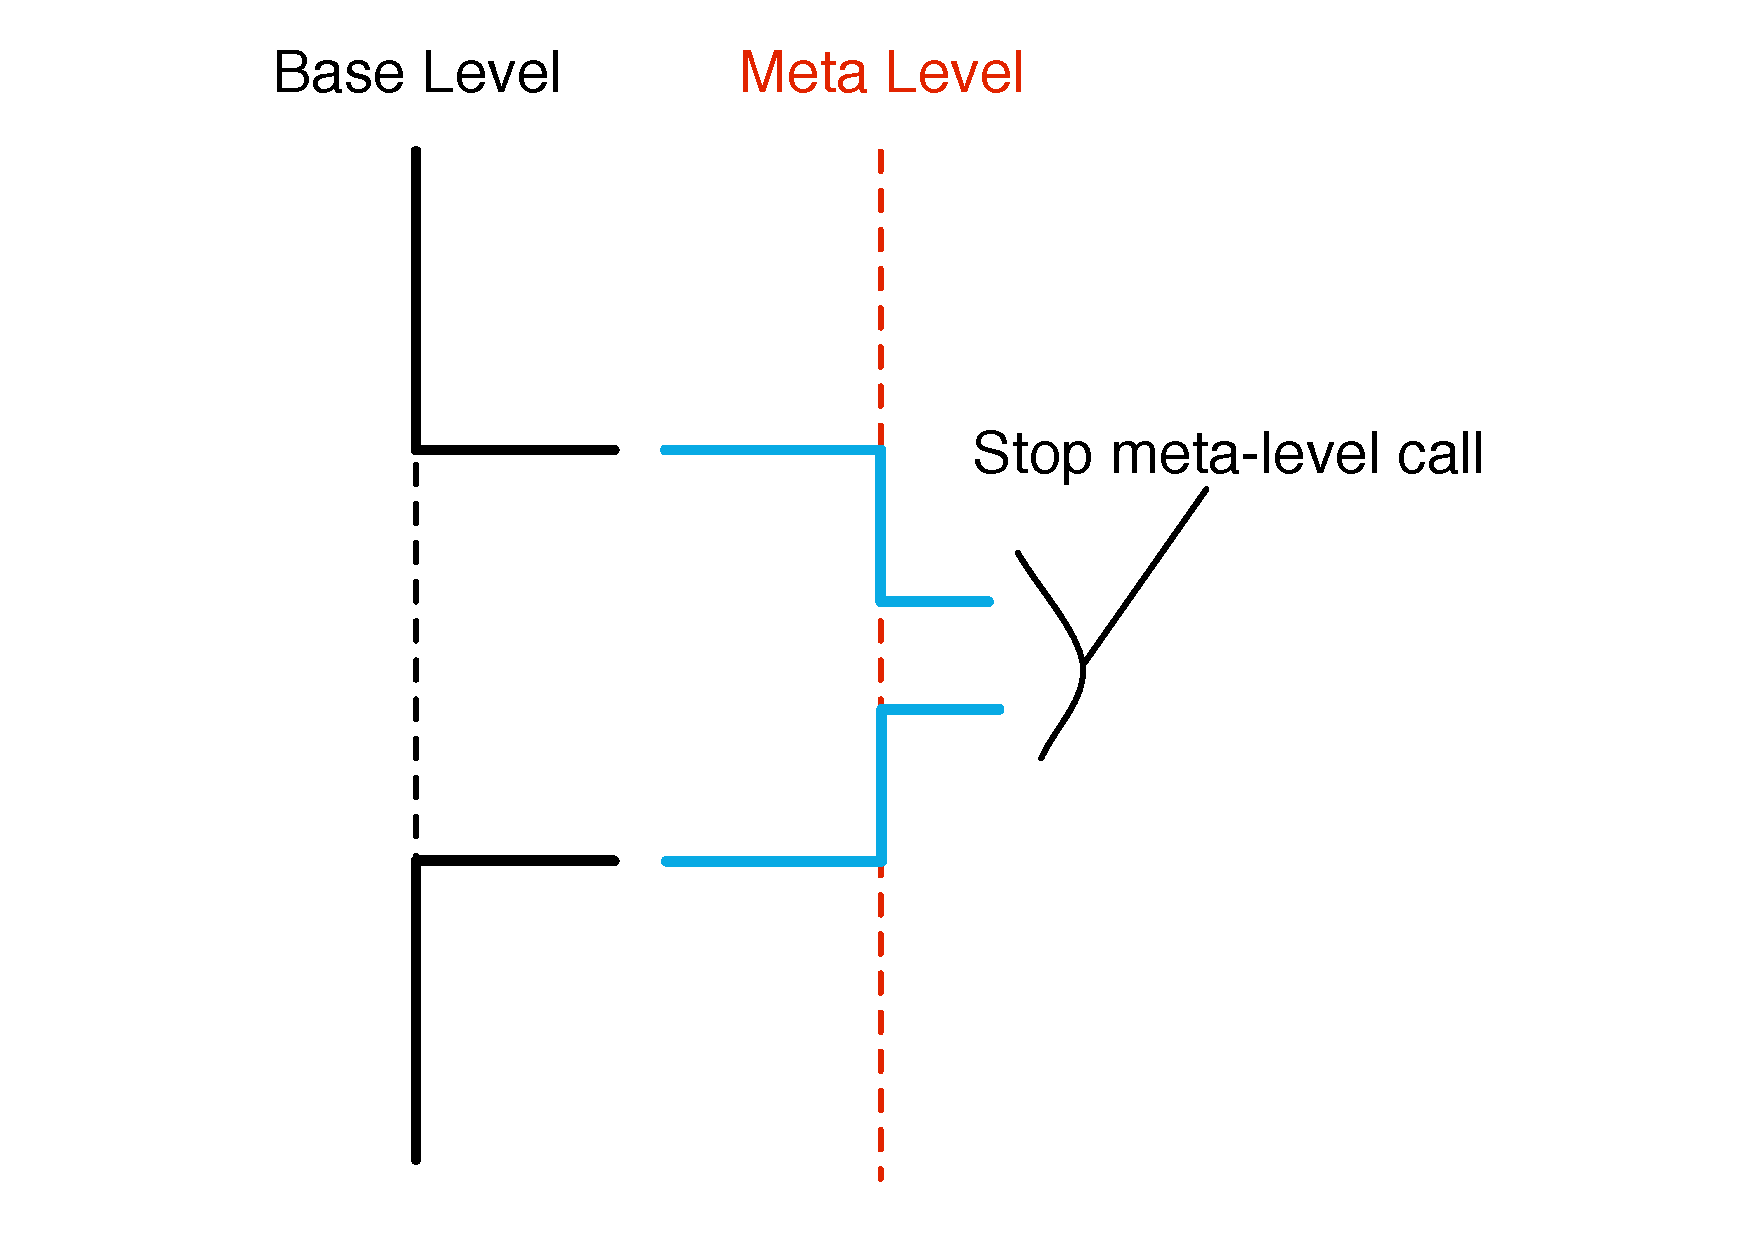
\includegraphics[width=1\linewidth]{reflectivity_avoid_recursion}
\end{subfigure}
\caption{\textbf{Meta level jump using reflectivity.}\label{fig:reflectivity_avoid_meta_recursion}
% (a)The host language and (b)the guest language contain each one their own classes and objects. The guest language resides inside the host language during the bootstrap; (c)the builder, a program written in the host language, reifies the bootstrap process itself and bootstraps the guest language given a (d)source code specification.
 }
\end{center}
\end{figure}

Reflectivity succeeds to modify and scope behavioral reflection for different meta-levels inside a single interpreter reflective architecture. However, it does not provide support to fully change the language semantics~(residing in the \VM) or to perform structural reflection.

\section{Metacircular Runtimes and \VMs}\label{sec:metacircular_runtimes}

The increased complexity of the \VMs leads to more novel approaches on how to build \VMs and therefore, their runtimes.
Metacircular \VMs are \VMs programmed in the same language they support in the end \eg a Java \VM written in Java or a Smalltalk \VM written in Smalltalk. This approach is based on the principles of \emph{high-level low-level programming} \ie expressing low-level concerns using high-level languages~\cite{Fram09a}. Metacircular \VMs benefits from the abstraction power and tooling of a high-level language to manipulate their own \VMs. This also means that during the build-time of a metacircular \VM, we can express the manipulations of its application runtime in terms of the high-level language.

However, these projects are biased towards \VM building techniques and not to the manipulation of the application runtimes that run on top of them. We can see this in the fact that most of the high-level manipulations inside a metacircular \VMs do not survive the \VM generation \ie once the \VM is built we cannot access its high-level representations any more.  Even if we do not focus on the modification of \VMs, in this thesis we briefly study metacircular runtimes and \VMs with the objective of understanding more concretely the benefits of their high-level low-level approach.

\subsection*{\textsc{Squeak Smalltalk \VM}}
\seclabel{background-squeak}
% ---------------------------------------------------------------------------
The Squeak \VM~\cite{Inga97a} is an early open source metacircular \VM for the Smalltalk language. 
Its core building system is still in active use for the \urlfootnote{Cog \VM}{http://www.mirandabanda.org/cogblog/} which introduces a JIT compiler.
The Cog \VM is used as default by the \urlfootnote{Pharo}{http://pharo.org/} programming language.
The Squeak \VM is developed using a Smalltalk subset called Slang that is exported to C to be compiled to the final \VM binary.
%Additionally, the Slang sources can be interpreted to provide an interactive simulator of the \VM, including full graphical support.

Slang is limited to functionalities that can be expressed with standard C code.
Slang in this case is mostly a high-level C preprocessor.
Even though Slang basically has the same syntax as Smalltalk, it is semantically constrained to expressions that can be resolved statically at compilation or code generation time and are compatible with C.
Hence Slang's semantics are closer to C's than to Smalltalk's.
Unlike later metacircular frameworks, the Squeak \VM uses little or no compile-time reflection to simplify \VM designs.
However, class composition helps to structure the source code.
Next to the Slang source code which accounts for the biggest part of the interpreter code, some operating system related code and plugins are written in C.
To facilitate the interaction with the pure C part, Slang supports inline C expressions and type annotations.

A great achievement of the Squeak \VM is a simulator environment that enables programmers to interact dynamically with a simulated version of the running \VM.
The simulator is capable of running a complete Squeak Smalltalk image including graphical user interface.
This means that programmers can change the sources of the running \VM and see the immediate effects in the simulator.
The \VM developer has complete access and control to the \VM internals and the application runtime it contains. It can, for example, change any object and class inside the simulated application runtime. However, to apply such a change it depends on a memory-oriented interface \ie object modification is achieved by a Smalltalk interface that provides C-like abstractions such as pointer arithmetics. Additionally, once the \VM is generated, this low-level interface disappears and it is not accessible for the developer anymore.

% ---------------------------------------------------------------------------
\subsection*{\textsc{Jikes: High-level low-level Programming with MMTK}}
\seclabel{background-jikes}
% ---------------------------------------------------------------------------
Jikes (formerly Jalapeño) is an early metacircular research \VM for Java written in Java~\cite{Alpe00a}.
The Jikes \VM features several different garbage collectors and does not execute bytecodes but directly compiles to native code.
With metacircularity in mind Jikes does not resort to a low-level programming language such as C for these typically low-level \VM components.
Instead they are written in Java as well using a high-level low-level programming framework.
The Jikes \VM had performance as a major goal, hence direct unobstructed interaction with the low-level world is necessary using a specialized framework.
%High-level low-level programming \cite{Fram09a} is mentioned the first time in the context of the Jikes \VM project.
%The goal of high-level low-level programming is to provide high-level abstractions to simplify low-level programming.
%Essentially this is the same motivation that drives the metacircular \VM community.

Frampton et al. present a high-level low-level framework packaged as \ttt{org.vmmagic}, which is used as a system interface for Jikes. This framework introduces highly controlled low-level interaction in a statically type context. This framework provides a memory-oriented API to manipulate runtime entities at \VM generation time, which is used to implement \VM concerns. Once the \VM is compiled to native code, the interface exposed by the \ttt{org.vmmagic} framework is also compiled into native code and not accessible from Java programs executed on the top of the Jikes VM.


% ---------------------------------------------------------------------------
\subsection*{\textsc{Maxine Java \VM}}
\seclabel{background-maxine}
% ---------------------------------------------------------------------------
Maxine is a metacircular Java \VM~\cite{Wimm13a} focused on an efficient developer experience.
Typically \VM frameworks focus on abstraction at the code-level which should yield simpler code and thus help reducing development efforts.
However, in most situations the programmer is still forced to use existing general purpose tools for instance to debug the \VM.
In contrast, the Maxine \VM provides dedicated tools to interact with the \VM in development.
Maxine uses abstract and high-level representations of \VM-level concepts and consistently exposes them throughout the development process.

The Maxine project follows an approach where reflection is used at compile-time \ie once the \VM is generated, the metacircular property of the \VM is lost. However, during development Maxine tools provide a live interaction with the complete state of the running \VM artifact while debugging it.

%\subsection*{\textsc{PyPy Toolchain}}
%\seclabel{background-pypy}
%% ---------------------------------------------------------------------------
%\urlfootnote{PyPy}{http://pypy.org/} is a Python-based high-level \VM framework~\cite{Rigo06a}.
%PyPy's major focus lies on an efficient Python interpreter.
%However, it has been successfully used to build \VMs for other languages including Smalltalk~\cite{Bolz08a}.
%Interpreters are written in a type-inferable subset of Python called RPython.
%The underlying PyPy infrastructure automatically provides memory management and JIT compilation.
%Instead of explicitly providing these features, a \VM developer hints certain information to the PyPy framework to improve the generation of a GC or JIT.
%
%PyPy follows a different approach from the previously presented \VM generation frameworks.
%For instance, in Squeak and Jikes the final \VM implementation is not much different from an implementation done directly in a low-level language.
%The programmer specifies all the components of the \VM explicitly, either by implementing them directly or using a provided library.
%Compared to the more static C and C++ these \VM generation frameworks make the compilation phase more tangible.
%Smalltalk in Squeak or Java in Jikes or Maxine fulfill the purpose of the template system in C++ or the restricted macro system in C.
%For the explicit implementation part PyPy is no different.
%However, certain features for the final \VM are directly absorbed from the underlying PyPy infrastructure.
%For instance, the JIT support or the GC are not explicitly implemented but provided by the PyPy framework itself.
%This is a big difference to the other \VM frameworks as it allows programmers to write the \VM in a more high-level fashion.
%For instance in Squeak memory allocation, even for \VM-level objects, has to be performed explicitly.
%Whereas in PyPy the garbage collection is left to the underlying \VM building infrastructure.
%This approach allows RPython \VMs to behave like standard Python programs.
%
%Much like the automatic memory management, PyPy provides a tracing JIT generator~\cite{Bolz09a}.
%By default the \VM programmer does not write an explicit JIT in PyPy.
%Instead the \VM code is annotated to guide the underlying tracing JIT generator.
%This means a \VM compilation time a specific tracing JIT is created for the given meta information.
%As a result, the JIT can track high-level loops in the final interpreted language.
%Again, this is similar to PyPy's GC, both are provided as a service and do not have to be programmed explicitly.
%Instead, the \VM programmer tweaks parameters of the JIT or GC.

% ------------------------------------------------------------------------------
%\subsection*{\textsc{Pinocchio \VM}}
%\seclabel{background-Pinocchio }
%
%Pinocchio~\cite{Verw11a} is a research Smalltalk environment that directly uses native code instead of bytecodes.
%The only execution base is native code which is directly generated by the language-side compiler.
%
%Pinocchio is built from a kernel derived originally from a \PH image.
%For the bootstrap classes, objects and methods are exported into binary, native images and linked together with a standard C linker to a final executable.
%For simplicity it relies on a very small part of C code to provide essential primitives, for instance used for file handling.
%Additionally it specifies part of the bootstrap for the Smalltalk object model in plain C code.
%However, besides that, all the other code is written and developed directly in Smalltalk.
%
%An important aspect of Pinocchio is that the method lookup is expressed in terms of normal Smalltalk code.
%Typically this code statically resides in the \VM, thus at a different meta-level.
%Hence this implies for most systems that the lookup can not be modified without altering the \VM itself.
%However, expressing the lookup in terms for normal language-side code introduces a recursive dependency during the bootstrap.
%In order to run the lookup code expressed in Smalltalk code, we have to perform message sends.
%These, in return, require an already working lookup mechanism.
%Hence, without taking special care, a language-side lookup method will lead to infinite recursion during startup.
%Pinocchio resolves this problem by directly interacting with the low-level execution format which among other things relies on inline caches to improve performance.
%The important property of inline caches is that they bypass the slow language-side lookup by directly jumping to the last activated method at a send-site.
%This is exactly the behavior we need to prevent recursion during the startup.
%Hence, when generating the native code for the bootstrap, it prefills all the inline caches of the methods required to perform a full method lookup.
%As a result, when at runtime it is required the first real method lookup, the lookup code itself is running perfectly on the prefilled inline caches.
%Pinocchio achieves a flexible connection between the low-level world and the high-level language-side.
%During execution, the \VM jumps freely between what previously was native \VM-level code and interpretation of language-side code.

% ------------------------------------------------------------------------------
\subsection*{\textsc{Klein \VM}}
\seclabel{background-klein}

\urlfootnote{Klein}{http://kleinvm.sourceforge.net/} is a metacircular \VM for the Self programming language that has no separation into \VM and language \cite{Unga05a}.
A main difference between Klein and the already seen metacircular \VM projects is that the reification of the \VM-level elements survives the code generation or compilation time.
Instead the \VM structures are exposed to the language as Self objects, exposing them to the language and thus allowing their manipulation from the application runtime.
Klein also supports advanced mirror-based~\cite{Brac04b} debugging tools to inspect and modify a remote \VM.
%Hence the Klein \VM supports true \VM-level reflection since there is only a single code base.

Additionally to the advances in reflection and metacircularity, Klein focuses on fast compilation turnarounds and incremental modifications for a responsive development process.
For comparison, the generation process of a Squeak \VM takes minutes on modern hardware. The long compilation time prevents the Squeak \VM developer to perform fast and incremental development cycles on the \VM.

Development on the Klein \VM stopped in 2009 and left the Klein \VM in a fairly usable state.
Yet, it proved that it is possible and build a language-runtime without the classical separation of the language-side and the \VM.
From the literature presented about the Klein project we see a strong focus on the improvements of the development tools.
%The fact that the language-runtime allows \VM-level reflection to change the \VM dynamically is not directly mentioned in the literature.
%While we see the practical limitations of changing the \VM runtime system at runtime we would like to open the doors to this new form of reflection.

\section{Language Virtualization Techniques}\label{sec:background_virtualization_techniques}

The most related family of work in virtualization are approaches like Xen~\cite{Chis07a}. Xen is a Virtual Machine Monitor~(VMM) that allows one to control and manage \VMs in a high performance and resource-managed way. This approach targets the virtualization of full and unmodified operating systems~(OSs), to facilitate their adoption in industrial/productive environments. They rely on support from the hardware platform, and in some cases from the guest OS, concentrating themselves on performance and production features.

Operating System virtualization technology is characterized by the existence of a \emph{hypervisor}~(named after the Operating System \emph{supervisor} that controls the OS processes). The hypervisor is the \VM component that allows one to observe or control the internals of one or many \VMs. A \VM hypervisor gives us, amongst others, the following services:

\begin{description}
\item[Co-location.] Co-location is the ability to have co-existing applications on top of the same virtual machine. 
Co-located applications can use shared memory to communicate efficiently as they reside in the same operating system process.

\item[Resource control.] \VMs should control how the different resources of their applications are used. However, state of the art \VMs only control their consumed memory with the usage of a memory manager. They do not perform in general any control in other kind of resources such as CPU or energy consumption.
\item[Security.] \VMs should control how applications access sensitive information such as files and network connections or execute potentially dangerous operations such as system calls.
\item[Application mobility.] As applications are portable, they should be easily migrated between different \VMs also at runtime. Application mobility provides support for resource re-allocation.
\end{description}

High-level languages abstract the developer from the complexities of the underlying machine by running on top of a language \VM. A language \VM provides a language with an execution model closer to its semantics as well as several services such as automatic memory management or cross-cutting optimizations. Language \VMs also provide portability \ie a program can run on different operating systems and hardware architectures because the \VM abstracts it from the underlying particular details. Although these language \VMs are indeed \emph{Virtual}, state of the art production-ready \VMs do not provide by themselves the typical advantages of virtualized operating systems such as co-location, resource control, mature security or application mobility support.

With the objective of doing application runtime manipulation, we study in the following subsections techniques that to our understanding are virtualization-related techniques applied to application runtimes: application co-existence and application manipulation%. Finally, we conclude by presenting the aspects of these solutions that inspired our solution following in the next chapters.%We divide theses works in two main topics that are of interest for us in the subject of runtime manipulation. First, we present related work that targets co-location of language runtimes on the same \VM. We continue this section by presenting related work on the subject of runtime control.

%\subsection{Application Co-existence}\label{sec:virtualization_coexistence}

\subsection*{\textsc{Class Loaders}}
In Java, application co-existence can be achieved to some degree with class loaders. A class loader is a first-class entity responsible for dynamically loading classes: creating their runtime representation, loading their methods and linking their class references~\cite{Lian98a}. A class loader remembers all classes it loaded, and it is responsible for loading all classes they depend on. Class loaders define namespaces: different class loaders can load classes with the same name. These classes will be isolated in the sense that they will not be visible to the others statically.

Class loaders can be specialized and extended to provide custom behavior. For example, Fong et. al.~\cite{Fong10a} use the class loading mechanism to enforce scoping rules and determine the visibility of names in various region of the program. They allow the user to control untrusted
namespaces and classes and they have defined a language to define security policy. Jensen et. al.~\cite{Jens98a} provide a formalization of the class loader with the means to enforce security. They also use a bytecode verifier on class loading to check if a class' bytecode doesn't try to perform overflow or underflow operations.

In the context of this thesis, we consider the class loader isolation mechanism as it can be used for application co-existence. Different versions of the same application can be loaded by different class loaders and be running at the same time. Class loaders present however a main limitation on the so called \emph{bootstrap class loader}: the literature does not explore the means to load~(and use) different versions of the main runtime classes of the language. Moreover, Java's bootstrap class loader is often implemented natively, and as such, we have no control on it from the language.

Notice additionally that class loaders provide only a load mechanism. Once we have several versions of the same application, it does not support the means to manage changes or updates of these applications. In this regard, the OSGI~\cite{OSGI} architecture implementations often make use of class loaders to load classes into separately isolated components and manage them in a higher level way.

\subsection*{\textsc{Changeboxes}}

Changeboxes~\cite{Denk07c} is a change model designed to encapsulate and scope changes. Its main purpose is to allow several versions of a system to co-exist at runtime \ie the existence in the same environment of different versions of the same classes and methods. In changeboxes, a \emph{changebox} is a first-class entity that encapsulates changes made on the language elements~(\eg classes and methods) and an executable version of the system with its changes applied. The system can contain many changeboxes at the same time, and applications can be scoped to run within different changeboxes. This notion of dynamically scoping an application to a changebox allows one to have co-existing environments~(\eg testing, development, production), increasing the developer's efficiency. Furthermore, it eases application update and migration to new versions, and reduces its update down-time as the application does not have to be stopped to be updated.

A Changeboxes prototype was developed in Smalltalk and its scoping mechanisms were implemented as follows:

\begin{description}
\item[Message send interception.] Message sends can activate different methods, within different changeboxes. A MethodWrapper~\cite{Bran98a} is placed instead of the method that has multiple versions, and it delegates the execution to the method that corresponds to the currently valid changebox.

\item[Class access interception.] Smalltalk resolves class names at compile time, inserting a reference to the given class inside the method's literal array. However, accessing a class yields different class objects within different changeboxes. To resolve this, class accesses affected by a changebox are postponed until runtime, and the code is recompiled in such a way: instead of putting the class inside the literal array, the class is dynamically looked-up from the class table when it is accessed.
\end{description}

The Changeboxes model proves sound to update and migrate application and framework classes. However, it has the main drawback of not affecting critical classes in the system. The Changeboxes prototype does not work on language runtime classes such as \ct{Array} or \ct{CompiledMethod} as the underlying infrastructure~(the VM) restricts the system to the existence of only one of them at the same time. The changes model does not provide a solution for this problem, as it focuses on application code update, leaving this as an open problem.

\subsection*{\textsc{Caja\textbackslash Cajita} - Object Capability Languages}

Caja~\cite{Mill08a} is an object-capability language~\cite{Levy84a,Mill03a,Spoo00a} subset of Javascript that pursues the safe co-existence of isolated Javascript scripts. Caja was conceived in the context of the web, where untrusted scripts can be loaded in any webpage and profit from any data available in the webpage. Caja defines a safe Javascript subset that removes elements from the language such as \ct{with} or \ct{eval} because their semantics are "strange" and in some cases unpredictable. Caja includes Cajita, a subset of Caja without the \ct{this} keyword. Caja is meant for transforming and migrating already existing Javascript code, while Cajita is meant for newly written code.

Caja works with a combination of static and dynamic techniques. First, a static verifier checks and transforms Caja code into sanitized Javascript. This sanitized Javascript contains runtime checks that complement the static verifications. All these changes are meant to avoid exploits and vulnerabilities from untrusted sources. Caja also adds some new features to the Javascript libraries with support to freeze objects and turn them immutable. 

To allow the safe co-existence of several scripts, Caja removes the Javascript global environment and replaces it by modules. Caja Modules co-exist transparently and can only access each other's data through an explicit and verified interface.
%
%\subsubsection*{\textsc{Worlds}}
%Worlds~\cite{Wart08a} provide a way to control and scope side-effects in Javascript. Side-effects are limited to a first-class environment.

%\subsubsection*{\textsc{Gemstone}}
%Gemstone \cite{Otis91a} provides the concept of class versions. Classes are
%automatically versioned, but existing instances keep the class (shape and
%behavior) of the original definition. Instances can be migrated at any time.
%Gemstone provides (database) transaction semantics, thus state can be rolled
%back should the migration fail.
%Gemstone's class versions extend the usual Smalltalk class evolution mechanism for robustness, 
%large datasets, and domain-specific migration policies. In contrast, ObjectSpaces target general 
%reflective access and bootstrap-like evolutions of code that is critical to the environment.

\subsection*{KaffeOS}

KaffeOS~\cite{Back00a} is a multi-application Java Runtime System that supports application co-existence, isolation and resource accounting. The KaffeOS runtime allows the isolated co-existence of Java applications so they cannot access each other's data, nor interfere in their execution. For this, the KaffeOS \VM performs CPU and memory accounting and prevents an application to starve others by consuming more resources than expected.

KaffeOS adds the process abstraction in the Java language, as in the sense of a process for an operating system. Each KaffeOS process owns a separate memory region~(a process heap) where its objects are allocated. Shared objects reside in special shared memory regions. A \emph{kernel heap} makes a distinction between code that runs in user mode or kernel mode. Regarding process communication, cross-process references become cross-heap references and are handled specially by the \VM. Resources are accounted and controlled at the \VM level for each process, so no process starves other processes.

KaffeOS lets several Java applications run side by side taking care of hardware resource consumption in addition of application's data. However, this solution is still limited with respect to base language classes. For example, the class \ct{java.lang.Object} must be shared between different processes to allow their communication because of the type system checks.

%J-Kernel \cite{Hawb98a} and Luna \cite{Hawb02a} present a solution similar to ours regarding the memory usage. They are Java solution for isolating object graphs with security purposes. In them, each object graph is called a \emph{protection domain}. All protection domains loaded in a system, and their objects, share the same memory space. 
%
%The J-Kernel enforces the separation between domains by using the Java type system, the inability of the Java language to forge object references, and by providing capability objects\cite{Levy84a,Mill03a,Spoo00a} enabling remote messaging and controlling the communication. This same separation in Luna \cite{Hawb02a} is achieved by the modification of the type system and the addition in the virtual machine of the \emph{remote reference} concept.

%\subsection{Application Manipulation}\label{sec:virtualization_control}

\subsection*{JVMTI}
The Java Virtual Machine Tool Interface~(JVMTI)~\cite{JVMPI} is the interface offered by the Java \VM for its manipulation and control. Originally called Java Platform Debugger Architecture~(JPDA) and used in the context of debugging, it was extended to support other use cases such as monitoring and profiling.
JVMTI exposes C functions to manipulate a Java VM~(Figure \ref{fig:jvmti}). The JVMTI client, so called an \emph{Agent}, queries and controls the given JVM through this interface. The manipulated JVM and an agent share the same operating system process. JVMTI agents are meant to be written in C, to be as compact as possible and allow maximal control with minimal intrusion.

\begin{figure}[ht]
\begin{center}
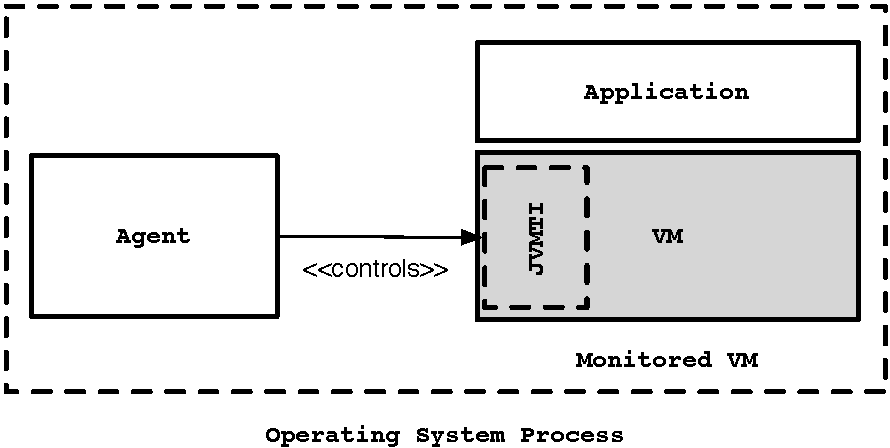
\includegraphics[width=.9\linewidth]{jvmti}
\caption{\textbf{JVMTI Architecture.} An agent controls a JVM though JVMTI. Both share the same operating system process.\label{fig:jvmti}}
\end{center}
\end{figure}

JVMTI provides introspection and some limited intercession facilities at the VM and language levels. In particular it provides memory and heap management, thread control, execution stack manipulation, object and class manipulation and breakpoint support. JVMTI is used mainly for debugging, monitoring and analysing purposes, particularly profiling and thread analysis.

In the context of this thesis, we identify in JVMTI's architecture a similarity to a virtualization system. The Java \VM takes the place of the virtualized operating system and the agent is its hypervisor.

\subsection*{MVM: a Multi User Virtual Machine}
The Multi-user Virtual Machine~\cite{Czaj03a,Czaj01a} is a general purpose virtual machine for the Java language that allows the co-existence of different applications, potentially from different users. Each application running on top of the MVM is an \emph{isolate} based on the Java Application Isolation API specification~\cite{JSR121}. This Java Application Isolation API defines a uniform mechanism to control the life-cycle of Java applications.

Many isolates co-exist not interfering with each other, as they believe they own their private JVM: the runtime is modified, so state is not shared between them by default. MVM allows several communication mechanisms to securely communicate between isolates: from standard mechanisms such as sockets, up to \emph{links}, a low-level isolate-to-isolate mechanism introduced by the Isolate API.

MVM can run unmodified Java applications. The main difference between MVM and other co-existence solutions is that MVM-aware applications can use its high-level API to control the life-cycle~(\eg creation, suspension, resuming and and termination) and the available resources of other isolates. Notice that differently from JVMTI, this control API is available to the applications running on the JVM and not only to native agents.

\section*{\textsc{Safe-Tcl}}
Safe-Tcl~\cite{Levy97a, Bore94a} is a variation of Tcl whose main purpose is the execution of Tcl scripts in a safe environment, with restricted permissions and attributions. Safe-Tcl achieves this by using co-existing \emph{twin interpreters} \ie a normal Tcl interpreter~(the master interpreter) can invoke another interpreter and specialize its behavior. Both the master and child interpreters run isolated from each other~(Figure \ref{fig:safetcl_twin_interpreters}).

\begin{figure}[ht]
\begin{center}
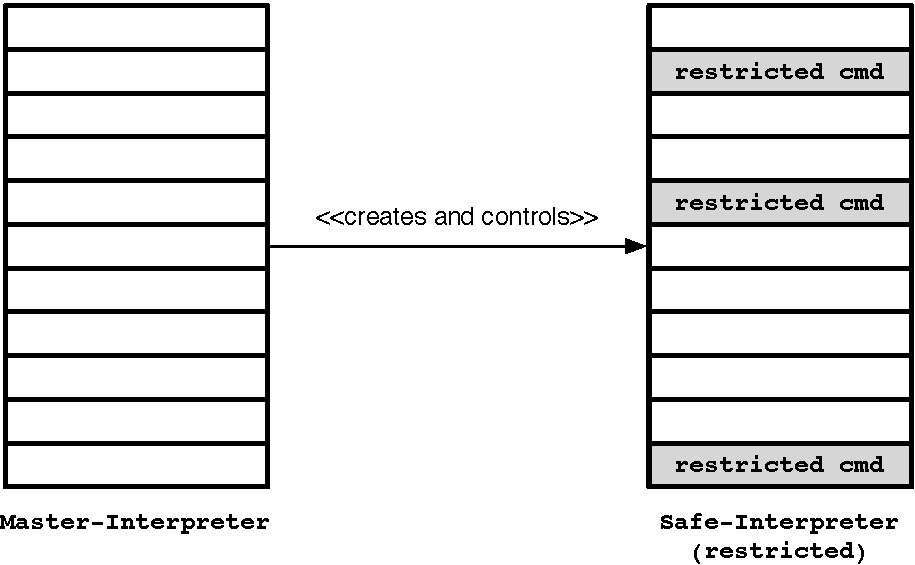
\includegraphics[width=.6\linewidth]{safetcl_twin_interpreters}
\caption{\textbf{SafeTcl Twin Interpretation.} The Master interpreter creates and configures a safe interpreter. The safe interpreter, with modified commands, will run the sandboxed Tcl application.\label{fig:safetcl_twin_interpreters}
% (a)The host language and (b)the guest language contain each one their own classes and objects. The guest language resides inside the host language during the bootstrap; (c)the builder, a program written in the host language, reifies the bootstrap process itself and bootstraps the guest language given a (d)source code specification.
 }
\end{center}
\end{figure}

The master interpreter modifies the behavior of a safe interpreter by providing a security policy. A security policy grants or removes privileges to the scripts executed on an interpreter. Commands can be aliased so the untrusted interpreter call an aliased method and the command is fully implemented by a trusted interpreter. The twin interpreter is an interesting solution to have co-existing independent application runtimes where one has the power to manipulate the second one at the level of the interpreter.

%Safe-Tcl twin interpretation allows us to change the behavior of a program running on a specialized interpreter, without the limitations of the infinite tower of interpreters. However, in contrast with the solutions we already presented, Safe-Tcl does not provide with the ability to change completely the semantics of the language but just to override or provide new commands, with a focus on security.

%\subsection*{Java Isolates}
%Java Isolates \cite{JSR121} allow multiple applications to run inside the same Java virtual machine.
%Nothing is shared between the different applications. Resources like CPU time, memory are controlled 
%and restricted. Isolates can communicate through channel, since nothing is shared the data are copied. 
%Java Isolates are defined in the Java Specification Request 121, but no commercials Java virtual 
%machine implement the specification.

% =============================================================================

\section{Conclusion and Summary}

In this chapter we studied the state of the art of application runtime manipulation techniques. We focus this study on three main concerns: the flexibility to change an application and language runtime, the mixture of low-level and high-level concerns and the tool support to do it. Based on these three concerns, we defined a criteria to present, evaluate and compare different work related to application runtime manipulation. We organized our state of the art in three categories: reflection models, metacircular runtimes and virtualization techniques. Table \ref{tb:comparison_runtime_manipulation} shows how our evaluation criterion match each of these categories.

\begin{table}[ht]
 \small
 	\centering
 	\begin{tabular}{lccccc}
	
\toprule
 			& \textbf{Reflection}
 			& \textbf{Metacircular}
			& \textbf{Virtualization}\\
% 			& \textbf{Dynamic} \\
 			& \textbf{}
 			& \textbf{Runtimes}
			& \textbf{Techniques}\\
% 			& \textbf{Analysis}\\
%  \cmidrule(r){2-4}
 \toprule

		Object Manipulation
 			& + & + & \textasciitilde \\
		\hline
		Language
		Manipulation
 			& + & + & \textasciitilde\\
		\hline
		Execution Manipulation
 			& \textasciitilde & + & + \\
		\hline
		Safety
 			& \textasciitilde & + & + \\
		\hline
		User Abstraction
		Level
 			& + & + & \textasciitilde \\
		\hline
		API Abstraction
		Level
 			& + & \textasciitilde & + \\
		\hline
		Separation of Concerns
 			& + & - & +\\
 	 \bottomrule
 	\end{tabular}
	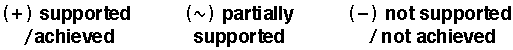
\includegraphics[width=.7\linewidth]{runtime_manipulation_criteria_overview}
 	\caption{Classification of application runtime manipulation into three different families of approaches and their evaluation based on the criteria defined in Section \ref{sec:runtime_modification_criteria}.}
 	\label{tb:comparison_runtime_manipulation}
 \end{table}

First, we studied different reflection and metaprogramming models such as the ones appearing in LISP, Smalltalk and Ruby. Metaprogramming and reflection support the modification of objects and language elements such as classes and methods. The reification of execution-related elements, though not always available, provides these models with the ability to also manipulate the execution: start, stop and alter the state of running processes. Reflection models require special support to safely apply arbitrary changes and not run into metastability issues \ie modifying an element that is used at the same time to make such modification can break runtime assumptions. Additionally, as reflection is available from the language, runtime manipulations are expressed in a high-level language. This provides the ability to both express our manipulations with high-level abstractions and to provide a high-level API to perform reflective changes. Finally, reflection support provides runtime manipulation separated from \VM concerns, as such support exists in the language.

Metacircular \VMs explore the idea of expressing a \VM in the same language it supports at the end, under the principles of \emph{high-level low-level programming}. High-level low-level programming aims at enhancing a developer's productivity by using the abstractions of high-level languages to express lower-level concerns. Metacircular \VMs have the same power as non metacircular \VMs: they can freely manipulate the application runtime that runs on them. They have the support for manipulating runtime objects, language and execution-related elements. Application runtime manipulations can be safely applied as they are atomic for the application runtime being executed. However, the main advantage of metacircular \VMs over regular low-level \VMs is that they are expressed in high-level languages and thus, we can express our manipulations with the expression power of such language. Not all metacircular \VMs provide an API written in terms of the runtime elements we want to manipulate, they do provide instead a memory-oriented API. Finally, metacircular \VMs do often mix language and \VM concerns, as they do not focus in the application runtime initialization but on the enhancements of \VM technology~(\eg the JIT compiler, the GC).

Virtualization techniques applied to application runtimes provide application co-existence and application runtime control. Application co-existence is used mainly with isolation purposes by allowing one to load several applications~(potentially several versions of the same application) to run at the same time and be able to communicate. These application co-existence solutions are provided to the high-level language developer. Application control solutions provide mainly support to control an application's life cycle: start, pause or stop it. They often provide an API expressed in terms of such elements, hiding the low-level details of such manipulations. Particularly JVMTI provides fine grained manipulation and control covering also object and language elements manipulations. Its main drawback is however that JVMTI agents are expressed in a low-level language, limiting the application of our solutions.

From this, we can state that our solution should have the following properties:

\begin{description}

\item[High-Level.] Expressing application runtime manipulations in a high-level language provides tooling support and a better level of abstraction for the developer of such manipulations. 

\item[Metaprogramming support.] Metaprogramming supports generally all kinds of manipulations that we desire for our solution. Making visible execution elements such as threads and the execution stack provides control over a program's execution.

\item[To manipulate a co-existing application runtime.] Manipulate a co-existing application runtime provides with the safety and atomicity of making such modifications from the \VM as it avoids to modify itself. Additionally, co-existing runtimes provide support to such manipulations from a high-level language runtime.

\end{description}

% =============================================================================
% =============================================================================
% =============================================================================

\chapter{Application Runtime Tailoring}
\chaplabel{state_tailoring}
\minitoc

Application runtime tailoring is the specialization of an application runtime so it contains only the elements necessary for its execution and no more. In other words, tailoring is a technique that generates a specialized application runtime so it can better adapt to devices with constrained memory.
This chapter starts by identifying the problem that motivates application tailoring: code bloat. Code bloat is mainly caused by unused code units appearing in general purpose libraries.
We illustrate this problem through an example~(Section \ref{sec:footprint_problems}).

Existing application extraction or \emph{Tailoring} techniques build deployment artifacts containing a subset of the original code units inside an application. However, these existing techniques are not completely efficient because they have to overcome many different challenges such as reflection or the absence of type annotations in dynamically-typed languages~(Section \ref{sec:challenges}). We present an evaluation criterion that allows us to compare these different existing solutions~(Section \ref{sec:tailoring_criteria}).

Finally, this chapter concludes by presenting and comparing existing techniques, grouped into four different categories: 
\begin{description}
\item[Dedicated platforms.] Pre-built tailored platforms with specialized \VMs and language runtimes~(Section \ref{section:static_selection_rw}).
\item[Static techniques.] Automatic tailoring techniques that depend only on static program information such as the source code and type annotations~(Section \ref{section:static_rw}).
\item[Dynamic techniques.] Automatic tailoring techniques that make use only of runtime information~(Section \ref{section:dynamic_rw}).
\item[Hybrid techniques.] Automatic tailoring techniques that complement both dynamic and static techniques~(Section \ref{section:hybrid_rw}).
\end{description}


\section{Problems of Deployment on Constrained Devices}\label{sec:footprint_problems}
Deployed object-oriented applications often contain \emph{code units}~(e.g. packages, classes, methods) that the running application never uses.
This problem is more evident and harder to control with third party software. 
Third party libraries and frameworks are designed in a generic fashion that allows multiple usages and functionalities, while applications use only few of them. 
Examples are logging libraries, web application frameworks or object-relational mappers.

Unused deployed code units have an undesired impact when targeting a constrained infrastructure. 
Some devices may constrain applications due to a restrictive hardware such as low primary or secondary memory~\cite{Mart12a}, or even software impositions such as the Android's Dalvik VM restriction to deploy only 65536 methods\footnote{According to dalvik's bytecode documentation~(\url{http://source.android.com/devices/tech/dalvik/dalvik-bytecode.html}), the source register accepts values between 0 and 65535.}. Big JavaScript mashup applications have an impact on loading time due to network speed and parsing time on the client.
These limitations may forbid the deployment of applications that contain lots of code units, or limit the amount of applications and content a user can have in its device.

Existing solutions to this problem eliminate dead code by extracting used code units of an application, and thus reduce application size in secondary memory and primary memory footprint. The majority of the solutions in the field automatically detect and extract used code units, so called \emph{tailoring}, with static call graph construction as the most dominant technique~\cite{Grov97a}. 
These static approaches present limitations in the presence of dynamic features such as reflection~\cite{Livs05a}, or in the absence of static type annotations. Additionally, they do not allow the user to customize the process of selection to cover different levels of an application's code \ie if third-party or base-language libraries are shared amongst several applications, a developer may want to extract only the used application specific code and leave the shared ones untouched; another developer may want to apply the process to the whole application.


%\section{A Motivating Example} \label{sec:example_intro}

\begin{figure}[ht]
\begin{center}
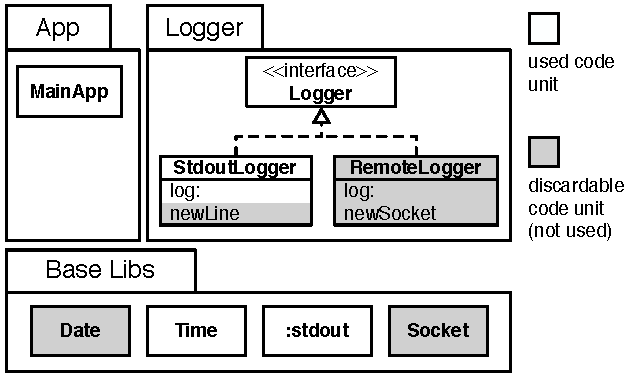
\includegraphics[width=.7\linewidth]{example_dead_code}
\caption{\small\textbf{Example of unused code units.} In gray, the unused code units that can safely be removed.\label{fig:example_dead_code}}
\end{center}
\end{figure}

To clearly show the problem, consider the application using a logging library in Figure~\ref{fig:example_dead_code}. In this figure, we emphasize in gray the unused code units that can safely be removed. Figure~\ref{fig:code_example1} shows the code of this application, written in the Pharo language. This application contains a \ct{MainApp} class with a \ct{start} method, which is the entry point of our application. The \ct{start} method creates an instance of \ct{Stdout\-Logger} and logs the application's start and end. In turn, the \ct{StdoutLogger} uses the \ct{stdout} global instance to log in the standard output the current time and the message. To print the time, the \ct{StdoutLogger} makes use of the \ct{Time} class from the base libraries of the language. Note that for the sake of clarity, we didn't include in the example all base libraries, though, in modern programming languages they represent a large codebase with several features going from networking to multithreading. For example, Java 8 SE contains 4240 classes\footnote{according to the javadoc API}, and the development edition of Pharo 3.0~\cite{Blac09a} contains 4115 classes and traits.
%An interface is present in the diagram to show polymorphism between two classes that do not share a class inheritance hierarchy. 
%However, some languages, such as the dynamically typed ones, may not need to represent it in the source code.

\begin{figure}[ht]
\begin{code}
MainApp>>start
    logger := StdoutLogger new.
    logger log: 'Application has started'.
    "do something"
    logger log: 'Application has finished'.

!\unusedcode{StdoutLogger>>newLine}!
!\unusedcode{~~~stdout newLine.}!

StdoutLogger>>log: aMessage
    stdout nextPutAll: Time now printString.
    stdout nextPutAll: aMessage.
    stdout newLine.
    
!\unusedcode{RemoteLogger>>log: aMessage}!
!\unusedcode{~~~| socket |}!
!\unusedcode{~~~socket := self newSocket.}!
!\unusedcode{~~~socket nextPutAll: Time now printString.}!
!\unusedcode{~~~socket nextPutAll: aMessage.}!
!\unusedcode{~~~socket newLine.}!

!\unusedcode{RemoteLogger>>newSocket}!
!\unusedcode{~~~"...."}!
!\unusedcode{~~~"creates an instance of socket given some configuration"}!
\end{code}

\caption{ \small\textbf{Code of the example logging application.} In gray, methods not used by the application.\label{fig:code_example1}}
\end{figure}

In this example we can detect the following unused code units, shown in grey in Figure~\ref{fig:example_dead_code} and Figure~\ref{fig:code_example1}:
\begin{enumerate}
\item The logger library includes two logging classes~(\ct{Stdout\-Logger} and \ct{RemoteLogger}). Only the \ct{StdoutLogger} is used and thus, the \ct{RemoteLogger} class can be discarded.
\item Since the \ct{MainApp} class does not use the \ct{Socket} class nor the \ct{RemoteLogger} class~(the only user of the \ct{Socket} class), the \ct{Socket} class can be discarded.
\item No class in the application makes use of the \ct{Date} class, and we assume for this example that it is not used in the base-libraries either. Then, this class can be safely removed.
\item The method \ct{newLine}~(lines 7-8 of Figure~\ref{fig:code_example1}) of the \ct{StdoutLogger} class is not used and can be also removed.
\item The \ct{StdoutLogger} class uses the \ct{Time} class to print the current time. Then, all code units that are not related to the \ct{Time now} resolution or printing~(\ie time arithmetic) could be considered as unused.
\end{enumerate}

We would like to generate a new version of this application not containing these unused code units while keeping the application's behavior. We call this process \emph{application tailoring}.

\section{Challenges of Application Tailoring} \label{sec:challenges}

A lot of work exists on the tailoring of statically-typed applications~\cite{Cour10a,Rays02a,Tip03a,Popa04a,Teod01a}, where type annotations aid in the resolution of which piece of code will be used at runtime. 
However, static analysis is not an option in the context of dynamically-typed languages or in the presence of meta-programming and reflection~\cite{Livs05a}.
%~\cite{Mart12a}
In this context of dynamically-typed and object-oriented programs that may use reflection, we identify the following main challenges in creating tailored applications:

\begin{description}

\item[Language Runtime Unused Code Units.] As the core point of this thesis, we would like to extract not only application code but also code that belongs to the language base libraries, including its core meta-model. For example, if metaclasses are not used in a program and the \VM execution model does not require them to exist, we could safely remove them. The same could apply to classes and metaclasses that are part of the base-language libraries.

\item[Dynamic typing.] Dynamically-typed languages cannot benefit from the most powerful static analysis due to the absence of type annotations. Name-based static analyses~(static analyses that build a simpler call graph based only on method names) can be used on them, but are not as efficient. Static techniques to detect code unit usage, such as call-graph analysis, need the support of more dynamic techniques \eg tracking runtime information, following the application's execution flow, or performing symbolic execution.

For example, an approach just following method names would not eliminate the \ct{asString} method from the \ct{Object} or \ct{String} classes in the following code, as it cannot predict that only the \ct{asString} method of the \ct{Integer} class is used.

\begin{code}
MainApp >> start
    100 print

Integer >> asString
    "the code to create a string from an integer"
    ...

Object >> print
    stdout nextPutAll: self asString

!\unusedcode{Object >> asString}!
!\unusedcode{~~~\textasciicircum self class name}!

!\unusedcode{String >> asString}!
!\unusedcode{~~~\textasciicircum self}!
\end{code}

\item[Polymorphism and inheritance.] Polymorphism in object-oriented languages allows a code unit to treat objects of different concrete types in the same way as soon as they share a common interface. Inheritance plays a similar role: any class can extend another class and provide different behavior while sharing a common API.
As a consequence, both polymorphism and inheritance make the behavior of a program more difficult to predict by just statically analyzing its code units~\cite{Taen89a}.

\item[Application runtime configuration.] Modern applications often contain libraries and frameworks besides their proper code. 
To make these different code units fit together, applications rely on big configurations. 
These configurations are usually present in configuration files looked up dynamically by the application. 
Based on these configurations, the dependency injection pattern is usually used to dynamically set up the application. 
This recurrent and standard process for configuring applications implies that static analysis will be inefficient to detect used code units without library-specific knowledge.

For example, an application configuration can be changed at any moment after deployment to use different code:

\begin{code}
MainApp >> start
    userService := self configuration classById: #UserService.
    users := userClass new getUsers.
    ...

"XML with the application configuration"
<appContext>
    <classes id="UserService" class="LocalUserRepository" />
</appContext>

"Use this one if using a remote repository"   
<appContext>
    <classes id="UserService" class="RemoteRestUserRepository" />
</appContext>
\end{code}

\item[Reflection.] Reflection makes static analysis inoperative by allowing an application to execute unanticipated pieces of code. 
Any \ct{String} resulting from a program execution or program configuration can denote a message send, the name of a class to be instantiated, or even a script to be executed. We refer to method invocations as message sends because they represent better from our understanding the dynamic property of the invocation. Reflection is indeed important to cover, since it is a broadly used tool in industrial applications with object relational mappers such as Hibernate\footnote{\url{http://hibernate.org/}} or Glorp\footnote{\url{https://sites.google.com/site/glorpsite/}} and web frameworks such as Ruby On Rails\footnote{\url{http://rubyonrails.org/}}, Struts\footnote{\url{https://struts.apache.org/}} or Seaside\footnote{\url{http://www.seaside.st/}}.

\item[Intrusive approaches.] Intrusive tailoring approaches require us to change the application source code by using different APIs or particular interfaces. For example, J2ME~\cite{JavaME} is a tailored version of the Java runtime libraries that presents different APIs than the default Java distribution. Using this kind of solution requires adapting the application's code to this particular infrastructure. This is not a suitable option when facing legacy code and already existing large code bases.

\end{description}

\section{Evaluation Criteria}\label{sec:tailoring_criteria}

This section presents properties that we consider the most relevant to evaluate techniques addressing the issue of unused deployment code units.

\begin{description}

\item[Base-Library Specialization.] A programming language contains several base libraries covering very common and generic code. Not all the code units in these libraries are used in every application. An ideal tailoring solution must tailor base libraries of the language to reduce an application's deployment memory footprint.

\item[Third-Party Libraries Specialization.] Applications use several third-party libraries and frameworks covering several aspects of application development such as user interfaces, persistence or publication of services. Third party libraries contain large code bases and many dependencies. Thus, an ideal tailoring solution must tailor third-party libraries and frameworks too.

\item[Legacy Code.] An ideal tailoring solution must be applicable on already existing applications and not require modifications on them, independently of the size of their code-base.

\item[Reflection Support.] An ideal tailoring solution must handle correctly reflective code and resolve the unanticipated code executions in the same way as the application would do during runtime.

\item[General Purpose Infrastructure.] An ideal tailoring solution must produce a version of the application that is able to run on the official production infrastructure~(such as the VM) without overhead.

\item[Configurability.] An ideal solution for tailoring an application must support many different levels of application. Some applications may not need to tailor base libraries because they are shared with other applications. However, tailoring base libraries may be useful on applications residing alone in constrained devices.

\item[Dynamic typing.] An ideal tailoring solution must be applicable and effective in dynamically-typed languages \ie with no type annotations.

\item[Minimality.] An ideal tailoring solution must succeed at selecting the minimal set of elements that a deployable application must contain. That is, it must not contain extra~(non used) code units.

\item[Completeness.] An ideal tailoring solution must guarantee that the deployable application contains all the elements it needs to run without failure in all its possible execution paths.

\end{description}

In the following sections we explore and compare four different categories of solutions that pursue minimizing application memory footprint through application tailoring. Such a comparison is based on the criteria presented in this section.

%The reduction of the deployment footprint of object-oriented applications has been subject of interest both in industry and research since many years. In such regard, we identified four different families of solutions for dead code elimination: dedicated platforms~(cf. Section \ref{section:static_selection_rw}), static analyses~(cf. Section \ref{section:static_rw}), dynamic analyses~(cf. Section \ref{section:dynamic_rw}) and hybrid analyses~(cf. Section \ref{section:hybrid_rw}).

\section{Dedicated platforms}%Pre-conceived specialized application-independent platforms}
\label{section:static_selection_rw}

Dedicated platforms are platforms containing frameworks and/or libraries customized to run under specific circumstances. For example, Java Micro Edition~(J2ME)~\cite{JavaME} is a dedicated version of the Java platform and Cocoa Touch is one for the Cocoa framework\footnote{\url{https://developer.apple.com/technologies/ios/cocoa-touch.html}}. These specialized platforms are reduced platforms to run applications inside mobile and constrained devices. These platforms provide a reduced and fixed set of base libraries defined \emph{a priori} and in a not customizable way. On one hand, this means that applications written for this platforms will never miss a code unit and fail at runtime. On the other hand, completeness comes at the cost of minimality: the final application includes more code units than the ones required at runtime.

Applications have to be written especially for and with these dedicated platforms. Thus, legacy code and third-party libraries not written with them are not compatible and cannot be deployed. Reflection is not a problem if the dedicated platform provides it. This is because the statically tailored base libraries are not built in an automatic fashion and the application code is not tailored.

\section{Static Analysis-Based Techniques}\label{section:static_rw}

Static analysis approaches for dead code elimination make use of the static information of a program to select the minimal subset of used elements. The bibliography describes four different algorithms to achieve this goal: unique name, class hierarchy analysis~(CHA), rapid type analysis~(RTA) and reachable members analysis~(RMA) \cite{Baco96a, Titz06a}. These techniques share a common approach. They select an application's entry point method and deduce the execution flow from the available static information. For example, they use the available type annotations and class and method names. This information is often used to build a call-graph~\cite{Grov97a}.

These techniques have been studied and applied in many environments and languages. Rayside et al.~\cite{Rays02a}, Jax~\cite{Tip03a} and the ExoVM System~\cite{Titz06a} propose application extraction tools using these techniques for Java applications. Sallenave et al.~\cite{Sall10a} apply RTA to produce smaller .NET assemblies for embedded systems. Bournoutian et al.~\cite{Bour14a} use CHA to optimize on-device Objective-C applications. Agesen~\cite{Ages96a} presents in his thesis a static technique applied to Self, a dynamically-typed language. To achieve this, Agesen uses type inference to obtain type information and use it to select which objects to extract.

In summary, these approaches are based on the static types found either in the source code or byte code. Thus, they are not applicable \emph{efficiently} on dynamic languages with no static type declarations \ie some code units whose usage cannot be anticipated by these techniques will stay even if they are really not used during the application execution. However, these solutions are valuable as they allow one to tailor base and third-party libraries, and legacy code. Their tailoring approach generates new deployment units that can run on the standard runtime infrastructure. The main drawback appears in the presence of reflection and configuration files, which will only work with a subset of reflective invocations through complementary analyses on the strings found in the source code. Also, existing solutions in this family lack the possibility to configure the level of tailoring, making it an "all or nothing" approach.

\section{Dynamic Analysis-Based Techniques}\label{section:dynamic_rw}

Dynamic analysis techniques use exclusively runtime information~(\ie execution flow, alive objects, execution statistics) to perform dead code elimination. Amongst these, we identify two different approaches: \emph{load on demand} and \emph{code collection}. Load on demand approaches detect during runtime whenever a class or method needs to be installed and request it from a server. Code collection approaches deploy the full application  and garbage collect unused code based on usage statistics. Most related work in this family share a common characteristic: these techniques are used inside ubiquitous computing systems \ie systems meant to be always connected\gp{cite}. Ubiquitous computing systems, as they are always connected, have a possibility to fallback and recover in the case of incompleteness. However, to focus here on the dead code elimination techniques, we will discuss the incompleteness recovery techniques in \chapref{chap:rfg}.

\begin{description}
\item[JUCE \cite{Popa04a,Teod01a}.] It is a platform for ubiquitous computing devices supporting code load on demand and code collection. First, it initializes a minimal running application and code is loaded, with a method granularity, from a server located in a different machine. At runtime, the code that is not used for some time is collected following usage statistics, and loaded back again on demand if needed.

\item[OLIE~\cite{Gu03a}.] It is an engine that intelligently partitions and offloads objects during runtime to minimize memory consumption. It is part of the adaptive infrastructure for distributed loading (AIDE). In OLIE, offloaded objects are indeed migrated to nearby remote devices. Migrated objects can be accessed later through proxies that perform remote invocations on them.

\item[SlimVM~\cite{Kers09a, Wagn11a}.] It is an ubiquitous computing system where all code resides on a remote server and is loaded only on demand on small devices. Some static analysis is performed only on the server to reduce the size of the transported code, by identifying most likely needed code. SlimVM changes the class format make it more compact and improve loading time. On the client side every code load is done dynamically.

\item[Marea~\cite{Mart12a}.] It is an application-level virtual memory for object-oriented systems based on code collection. Marea allows not only the collection of code units but also the collection of arbitrary objects with a graph granularity. Collected graphs are swapped out to disk and swapped in back when the program tries to access one of the objects inside the object graph. Marea is supported by an object serializer with focus on fast deserialization to enable swap in's with small performance overhead, and a small memory footprint proxy library. The main drawback of this solution is that it lacks the automatic detection of objects to swap out and requires support from the developer for this.

\end{description}

All solutions inside this category except for Marea share one main property: they require to run the application inside a dedicated infrastructure to apply their techniques \eg dedicated VMs implementing remote lazy loading, code collection or special bytecode sets. The main challenge of these solutions resides on applying these techniques while minimizing their impact on performance during the runtime. Additionally, these solutions require their applications to run exclusively inside their infrastructure. Contrastingly, Marea solves this challenges with minimal overhead by using the existing reflective features of Pharo.

Regarding dynamic features such as reflection, these solutions are the ones that can, potentially, handle it in the best way since they have in runtime all the information needed to resolve it. JUCE and OLIE and Marea, handle naturally reflection as they do not change the runtime representation (which programs make assumptions of, when they use metaprogramming). SlimVM on the other hand, had to change the reflection support because they changed the object and class representation on their VM.

Regarding its applicability, SlimVM needs to recompile the whole application into its own format; Marea needs some development support for the collection of object graphs; OLIE and JUCE can tailor base and third party libraries without any modifications on them. Thus, the latter two can be applied to legacy code also for free. From all of these solutions, Marea is the only one that provides the ability to select the level of tailoring by customizing the serialization of the object graph to be swapped out.

The minimality of these approaches depends on the granularity of their loading mechanisms and the effectiveness of their code collection techniques. Big loading granularities may load more code units than the used, preventing minimality. The same problem appears in the case of Marea, where the code collection is managed by the application and depends on its implementation.

\section{Hybrid Analysis-Based Techniques}\label{section:hybrid_rw}

Hybrid analysis techniques partially mix static and dynamic~(\ie run-time) information. Their common approach is to start an application and pause it after some minimal run-time information is available \ie call stacks are created, some classes are loaded and initialized, and some objects are instantiated. Then, it uses the built stack of alive objects to perform a static analysis, as described in Section \ref{section:static_rw}, with concrete type information. During the rest of the analysis, no more dynamic information is used.

Java in The Small (JITS)~\cite{Cour10a} uses a hybrid approach to select the used parts of a program, and then loads them inside a binary image. A dedicated VM loads the binary image at startup. JITS's approach tailors base and third-party libraries as well as application specific code. It does not require modifications on the existent application to tailor it, so a legacy application could theoretically be tailored with this approach. JITS does not offer the possibility to configure the tailoring level, since it was designed to be used only in embedded devices where no more than one application would be running. Regarding reflection, JITS presents the same drawbacks as the other static call graph analysis approaches since not all the runtime information about the reflective invocations can be deduced.

\section{Conclusion and Summary}

Tailoring is a cross-cutting process that may affect any element of an application runtime, and thus, it requires particular support to detect and extract used code units. Several existing techniques were applied in the past with several results.
Table~\ref{tb:comparison_intro} presents a comparison of these techniques, given the criteria we presented in Section~\ref{sec:tailoring_criteria}.

\begin{table}[ht]
 	\centering
 	\begin{tabular}{ccccc}
	
\toprule
 			& \textbf{Dedicated}
 			& \textbf{Static}
			& \textbf{Hybrid}
 			& \textbf{Dynamic} \\
 			& \textbf{platforms}
 			& \textbf{Analysis}
			& \textbf{Analysis}
 			& \textbf{Analysis}\\
 \toprule

		Base Libraries
 			& + & + & + & +\\
		\midrule
		Third-Party
		& & & & \\Libraries
 			& - & + & + & +\\
		\midrule
		Legacy Code
 			& - & + & + & \textasciitilde \\
		\midrule
		Reflection Support
 			& + & - & - & + \\
		\midrule
		General Purpose
			& & & & \\
		Infrastructure
 			& + & - & - & \textasciitilde  \\
		\midrule
		Configurability
 			& - & - & - & \textasciitilde   \\
		\midrule
		Dynamic typing
 			& + & - & - & + \\
		\midrule
		Minimality
 			& - & + & + & \textasciitilde \\
		\midrule
		Completeness
 			& + & - & - & \textasciitilde \\
\bottomrule
 	\end{tabular}
	
	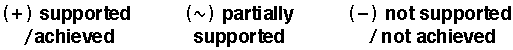
\includegraphics[width=.7\linewidth]{runtime_manipulation_criteria_overview}
 	\caption{Evaluation criteria applied to related work on deployment code unit tailoring techniques}
 	\label{tb:comparison_intro}
 \end{table}

Dedicated platforms are a first useful attempt to produce a specialized application runtime. They contain a pre-selection of base libraries that application developers must rely upon. Dedicated platforms are not tailored by an automatic process: that means that all the developed code will be part of the deployable distribution. This lack of automatic tailoring process means on one hand that the usage of reflection will not affect the result of the deployed artifact. On the other hand it means, however, that it does not offer the possibility to really tailor third-party libraries, legacy code nor even the developed application code. This is why we also consider dedicated platforms to ensure completeness while they are not as efficient to ensure minimality as other techniques.

We also see that automatic tailoring techniques, in contrast with dedicated platforms, base their tailoring on the existing application code: they can tailor base and third-party libraries as well as legacy code. Amongst them, dynamic-analysis based techniques, and hybrid-analysis ones in some grade, are able to handle reflective calls properly. We can see an almost general lack of support to configure whether a code unit should be subject to the tailoring or not.

Regarding minimality, automatic techniques are more efficient when they have more information at their disposal. Dynamic techniques use runtime information to know the concrete types of objects while static techniques use the types annotations in the source code. Between the two, dynamic techniques are more efficient because they benefit from more accurate information.

Concluding, it is important to notice that none of the automatic tailoring techniques ensure completeness by themselves. We cannot anticipate the use of reflection and other dynamic techniques in complex scenarios. For this purpose, several techniques such as lazy loading or remote calls can be used to complement tailoring techniques. \chapref{chap:rfg} explores a new dynamic tailoring technique based on \Vtt. We show how our technique succeeds to tailor even in the existence of reflection and adds configurability while others do not. 


\input{chapter-footer.tex}